\section{Results/Findings}


\begin{comment}
\begin{itemize}
    \item Key Results: Present your main findings clearly, using charts, graphs, or diagrams where necessary.
    \item Data Interpretation: Explain the significance of the results in the context of your research objectives.
    \item Unexpected Outcomes: Highlight any results that were unexpected and how they impact your project.
\end{itemize}
\end{comment}
%\newpage

%\section{Results/Findings}





%#################################################################


\subsection{Key Results}

We present the key empirical findings of our study, beginning with class distribution insights, followed by model performance based on \AUCone (\AUCtwos are calculated on the test set), and finally an analysis of the predicted recession probabilities over time.

\subsubsection{Inherent Class Imbalance}

A significant class imbalance is evident across all time frequencies, as shown in Figure~\ref{fig:class_imbalance}. Recession periods are underrepresented in comparison to non-recession periods (approximately 19\% recession) Such skewed distributions necessitate the use of class-balancing techniques (SMOTE, random undersampling, class weights and weighting factor ($\alpha$)) to mitigate bias in model training.


\begin{figure}[H]
    %\centering
    \raggedright
    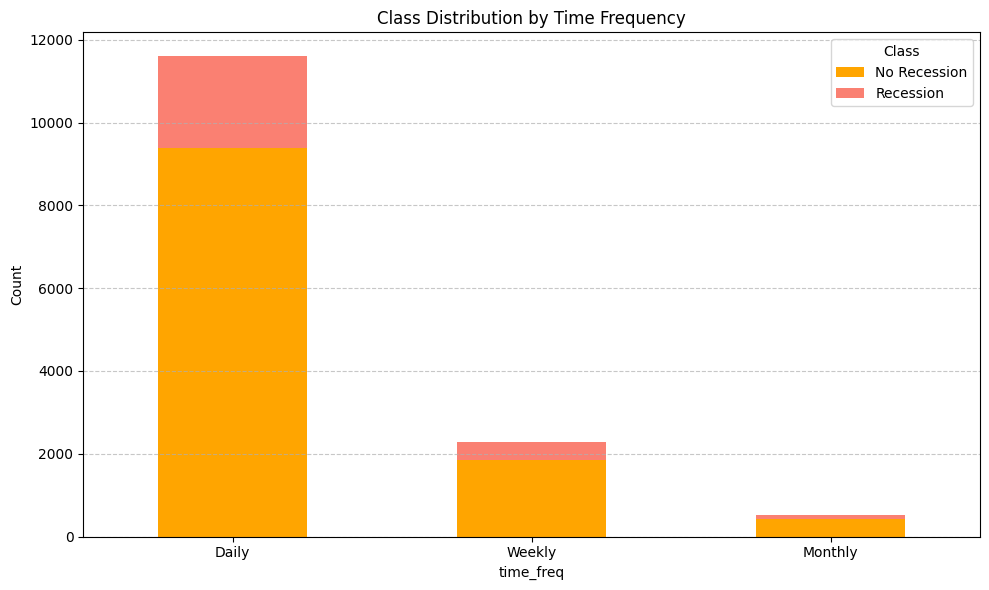
\includegraphics[
        width=0.6\textwidth,
        height=\textheight,%-24pt, 
        keepaspectratio
        ]
        {./Assignment/Final/Steps/Plots/png_class_imbalance.png}
    \caption{Stacked Bar Chart Showing Class Imbalance. 
    }
    \label{fig:class_imbalance}
\end{figure}

\vspace{-21pt}

\subsubsection{\AUCone Performance and Model Selection}

To evaluate model performance, we used \AUCone scores across each time frequency(daily, weekly and monthly). Traditional models with \AUCone scores below 0.5 (indicating worse-than-random performance) were excluded from further analysis, while all LSTM models were retained regardless of performance for comparison purposes.
As shown in Table~\ref{tab:auc_summary}, For traditional models, Logistic Regression and Easy Ensemble Classifier consistently achieved the highest \AUCtwos across all datasets. Logistic Regression performed the best with Easy Ensemble performing slightly lower but still comparable. Other Traditional models, including XGBoost, Balanced Random Forest, and traditional Random Forest, failed to reach the 0.5 \AUCone threshold in all scenarios.



\begin{table}[H]
\centering
\caption{\AUCone Scores by Model and Time Frequency (traditional models with \AUCone < 0.5 excluded; all LSTM models retained).}
\label{tab:auc_summary}
\begin{tabular}{lll}
\toprule
\textbf{Time Frequency} & \textbf{Model} & \textbf{\AUCone} \\
\midrule
Daily   & Logistic Regression       & 0.7222 \\
        & Easy Ensemble Classifier  & 0.6918 \\
        & \LSTMF                   & 0.7202 \\
        & \LSTMFF                & 0.7330 \\
        & \LSTME                   & 0.2752 \\
        & \LSTMEF                & 0.7291 \\
        & \LSTMEE                & 0.7021 \\
        \midrule
Weekly  & Logistic Regression       & 0.7251 \\
        & Easy Ensemble Classifier  & 0.6853 \\
        & \LSTMF                   & 0.7178 \\
        & \LSTMFF                & 0.7263 \\
        & \LSTME                   & 0.7604 \\
        & \LSTMEF                & 0.4078 \\
        & \LSTMEE                & 0.6019 \\
        \midrule
Monthly & Logistic Regression       & 0.7263 \\
        & Easy Ensemble Classifier  & 0.6675 \\
        & \LSTMF                   & 0.5335 \\
        & \LSTMFF                & 0.3880 \\
        & \LSTME                   & 0.3730 \\
        & \LSTMEF                & 0.5952 \\
        & \LSTMEE                & 0.4559 \\
\bottomrule
\end{tabular}
\end{table}


\subsubsection{Recession Probability Forecasts}
Figure~\ref{fig:table_lr_ee} 
displays the predicted probabilities of recession from the Logistic Regression and Easy Ensemble models across daily, weekly, and monthly datasets. 
Both Logistic Regression and Easy Ensemble models produce elevated probability estimates preceding known recession periods. 
Logistic Regression forecasts appear smoother and more gradual, the peaks appear less than 52 weeks to a recession, while Easy Ensemble produces sharper peaks about 52 weeks before a recession, indicating a greater sensitivity to abrupt changes in macroeconomic conditions.


%\renewcommand{\arraystretch}{0.5}
\begin{figure}[H]
    \raggedright
    \begin{tabular}{c c}
        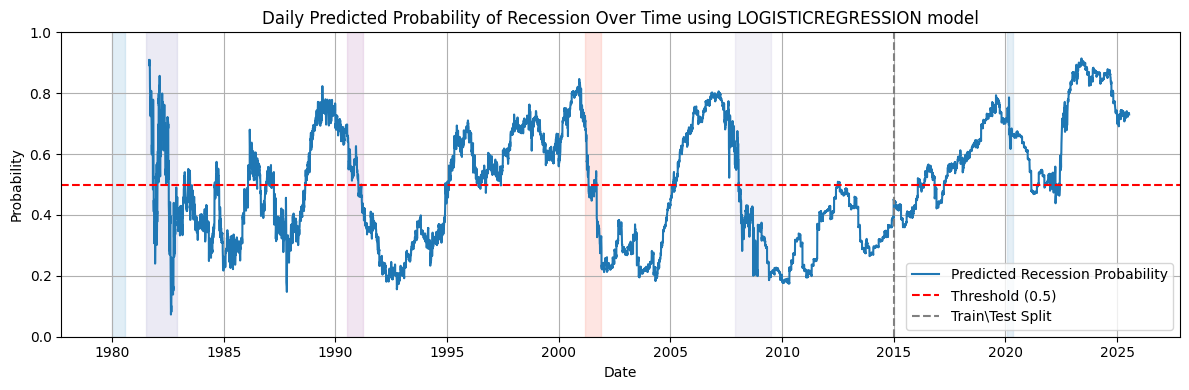
\includegraphics[width=0.48\textwidth]{./Assignment/Final/Steps/Plots/Daily Predicted Probability of Recession Over Time using LOGISTICREGRESSION model.png} &
        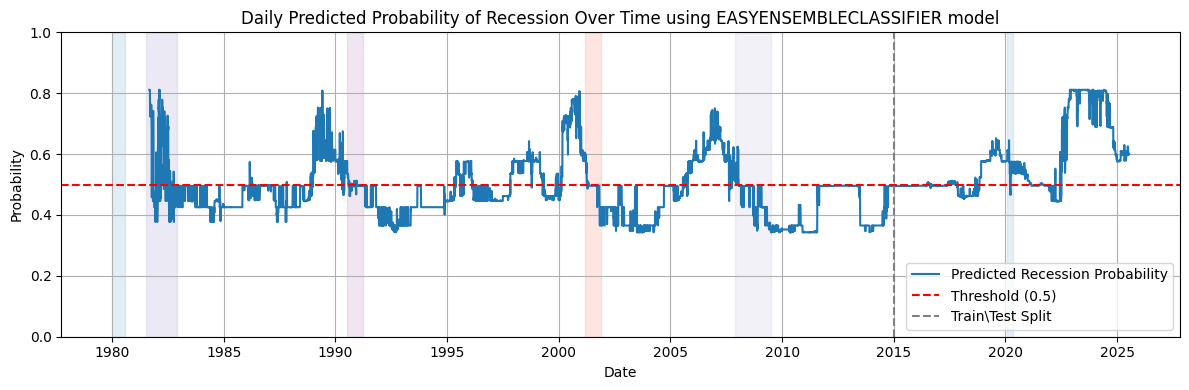
\includegraphics[width=0.48\textwidth]{./Assignment/Final/Steps/Plots/Daily Predicted Probability of Recession Over Time using EASYENSEMBLECLASSIFIER model.png} \\ [-9pt]
        %\textbf{Logistic Regression - Daily} & \textbf{Easy Ensemble - Daily} \\
        %\vspace{-9pt}
        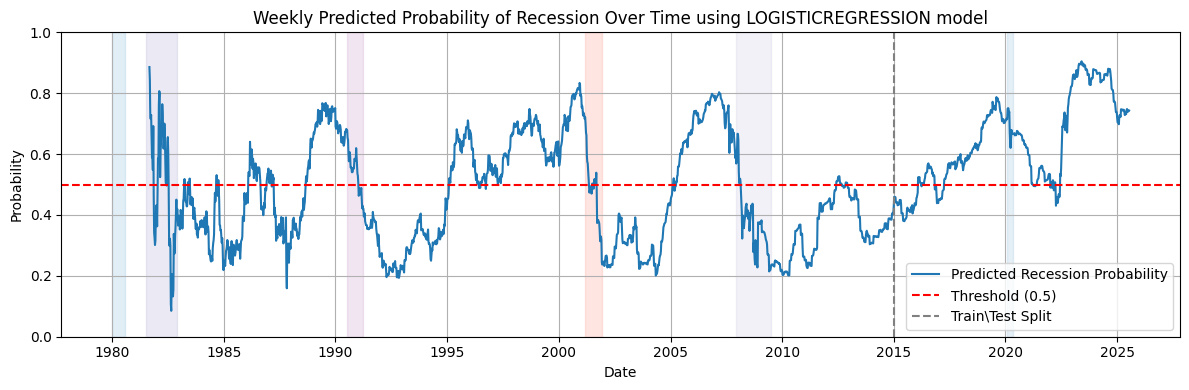
\includegraphics[width=0.48\textwidth]{./Assignment/Final/Steps/Plots/Weekly Predicted Probability of Recession Over Time using LOGISTICREGRESSION model.png} &
        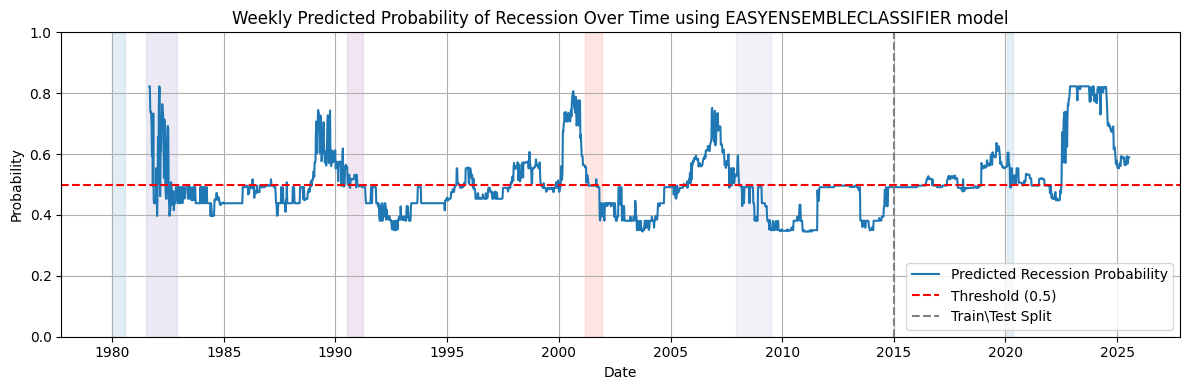
\includegraphics[width=0.48\textwidth]{./Assignment/Final/Steps/Plots/Weekly Predicted Probability of Recession Over Time using EASYENSEMBLECLASSIFIER model.png} \\ [-9pt]
        %\textbf{Logistic Regression - Weekly} & \textbf{Easy Ensemble - Weekly} \\
        %\vspace{-9pt}
        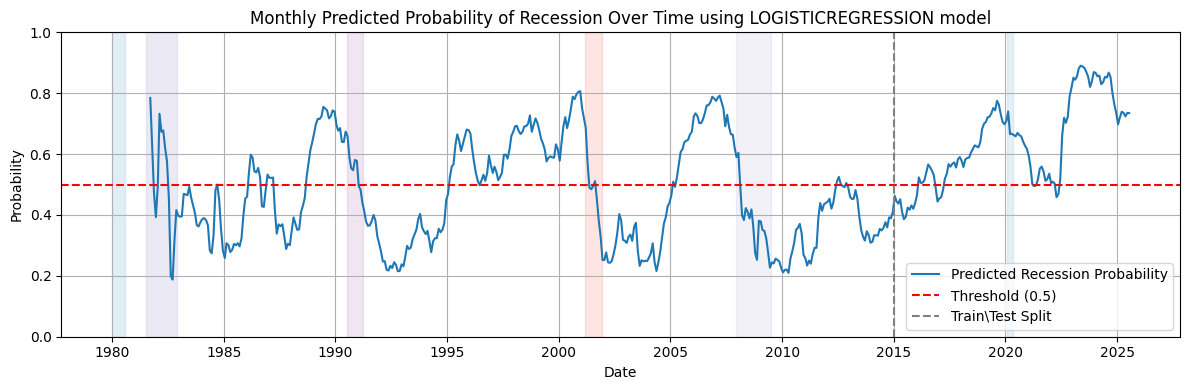
\includegraphics[width=0.48\textwidth]{./Assignment/Final/Steps/Plots/Monthly Predicted Probability of Recession Over Time using LOGISTICREGRESSION model.png} &
        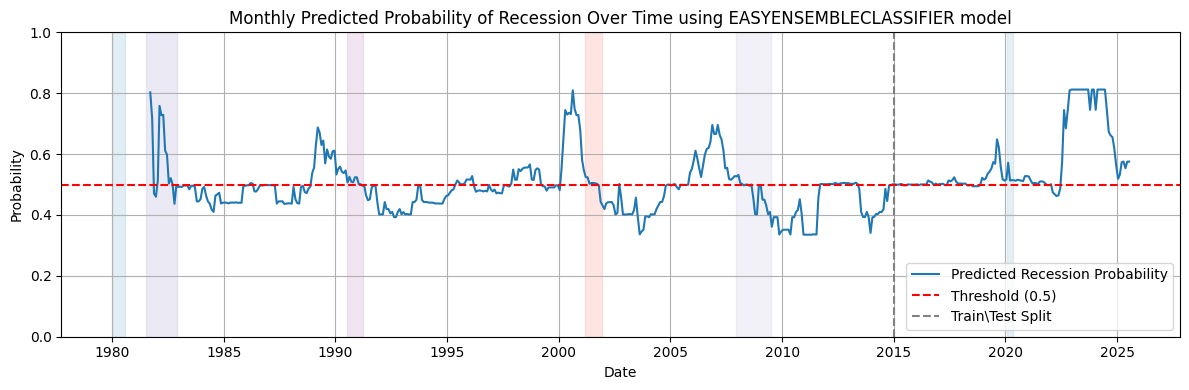
\includegraphics[width=0.48\textwidth]{./Assignment/Final/Steps/Plots/Monthly Predicted Probability of Recession Over Time using EASYENSEMBLECLASSIFIER model.png} \\
        %\textbf{Logistic Regression - Monthly} & \textbf{Easy Ensemble - Monthly} \\
    \end{tabular}
    \caption{Predicted probability of recession %across time frequencies 
    using Logistic Regression (left) and Easy Ensemble (right).}
    \label{fig:table_lr_ee}
\end{figure}

\vspace{-21pt}

To assess the forecasting capabilities of simpler deep learning architectures, we examined single-layer LSTM models in Figure~\ref{fig:table_lstm4_lstm8} (\LSTMF and \LSTME) across each time frequencies. 
At the daily forecasts, \LSTMF achieved moderate success (\AUCone = 0.7202), offering balanced sensitivity to changing conditions, while \LSTME performed poorly (\AUCone = 0.2752), displaying extreme volatility and a high rate of false positives. 
For the weekly level, \LSTME demonstrated the strongest performance (\AUCone = 0.7604), producing smooth and timely signals ahead of recessions. 
\LSTMF (\AUCone = 0.7178) showed sharper but more volatile responses, with better precision around recession windows, although it also exhibited random probability spikes between 1995–2000 and 2010–2015, similar to \LSTME, but more pronounced. 
On monthly data, \LSTMF yielded stable yet uninformative predictions (\AUCone = 0.5335), with probabilities remaining close to the 0.5 threshold, In contrast, \LSTME (\AUCone = 0.3730) tended to overreact to past recessions while downplaying periods of economic expansion.
Single-layer LSTMs showed varying degrees of effectiveness across time resolutions, with \LSTMF offering more consistent performance and \LSTME excelling only in the weekly setting but struggling at finer and coarser granularities.

\begin{figure}[H]
    \raggedright
    \begin{tabular}{c c}
        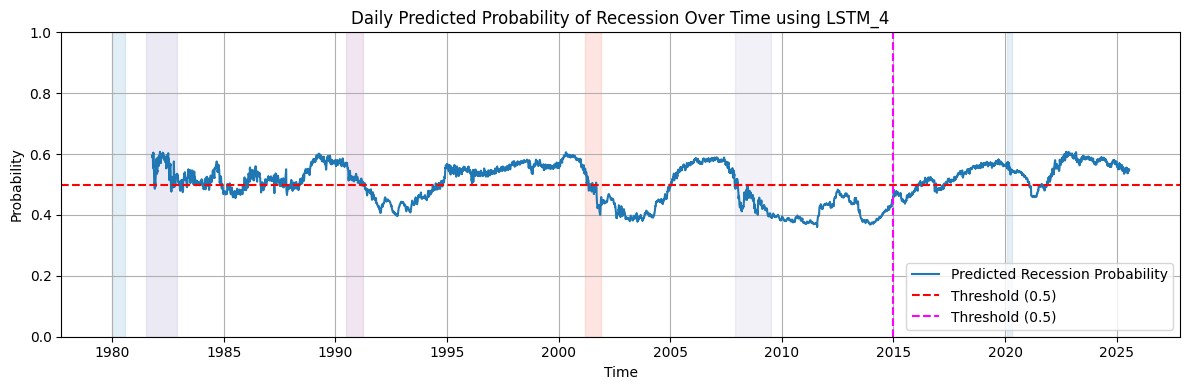
\includegraphics[width=0.48\textwidth]{./Assignment/Final/Steps/Plots/Daily Predicted Probability of Recession Over Time using LSTM_4.png} &
        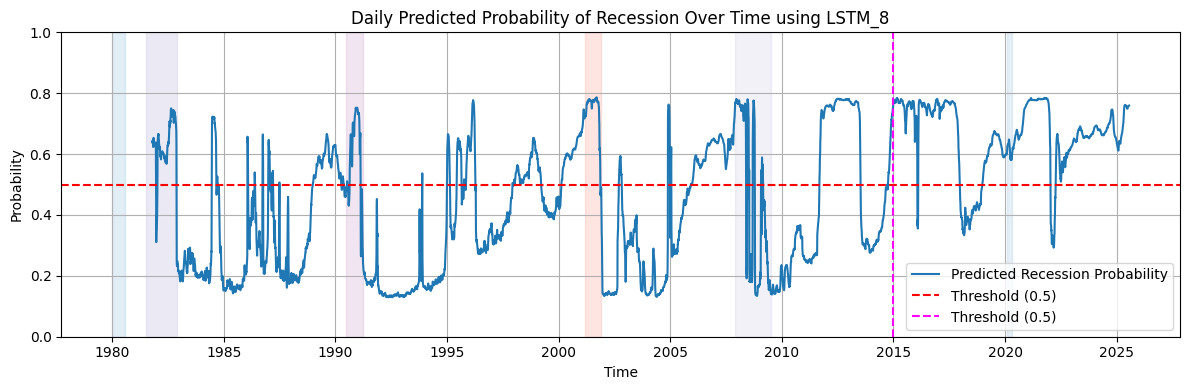
\includegraphics[width=0.48\textwidth]{./Assignment/Final/Steps/Plots/Daily Predicted Probability of Recession Over Time using LSTM_8.png} \\ [-9pt]
        %\textbf{Logistic Regression - Daily} & \textbf{Easy Ensemble - Daily} \\
        %\vspace{-9pt}
        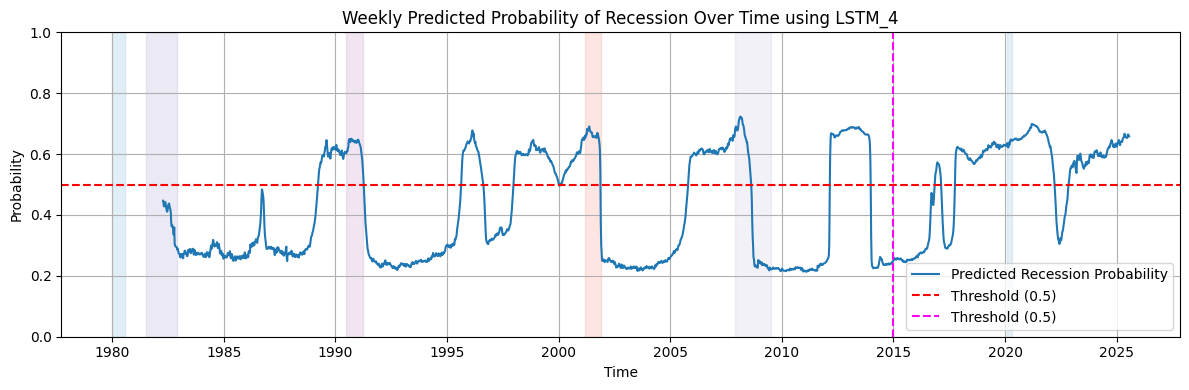
\includegraphics[width=0.48\textwidth]{./Assignment/Final/Steps/Plots/Weekly Predicted Probability of Recession Over Time using LSTM_4.png} &
        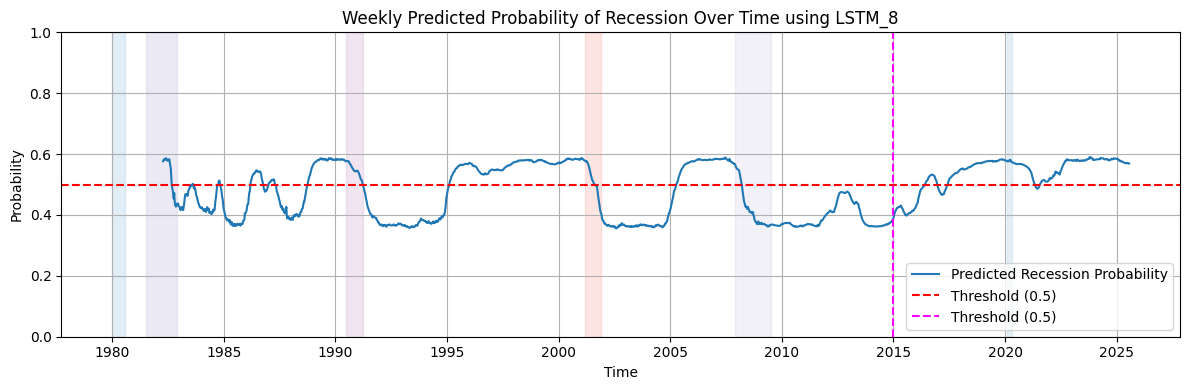
\includegraphics[width=0.48\textwidth]{./Assignment/Final/Steps/Plots/Weekly Predicted Probability of Recession Over Time using LSTM_8.png} \\ [-9pt]
        %\textbf{Logistic Regression - Weekly} & \textbf{Easy Ensemble - Weekly} \\
        %\vspace{-9pt}
        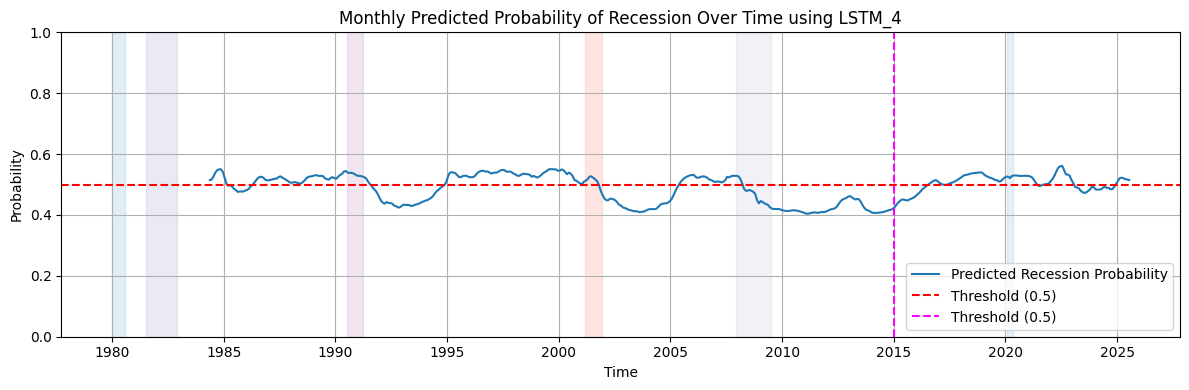
\includegraphics[width=0.48\textwidth]{./Assignment/Final/Steps/Plots/Monthly Predicted Probability of Recession Over Time using LSTM_4.png} &
        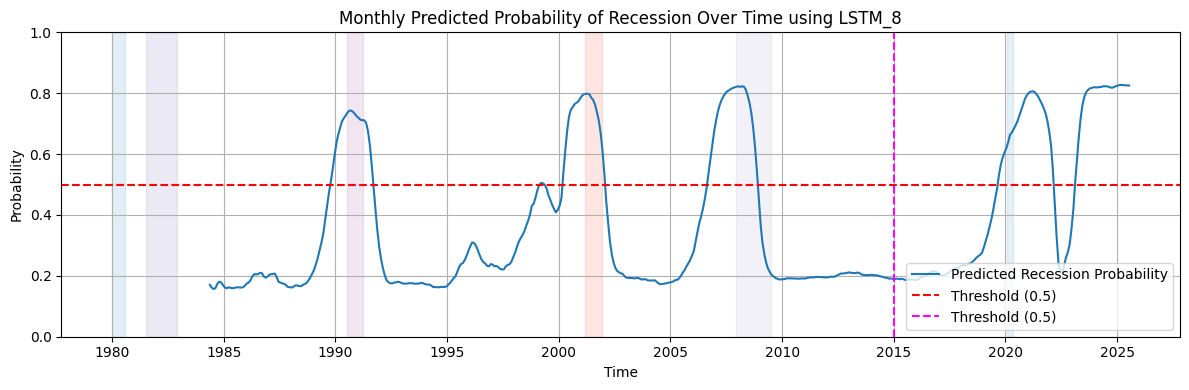
\includegraphics[width=0.48\textwidth]{./Assignment/Final/Steps/Plots/Monthly Predicted Probability of Recession Over Time using LSTM_8.png} \\
        %\textbf{Logistic Regression - Monthly} & \textbf{Easy Ensemble - Monthly} \\
    \end{tabular}
    \caption{Predicted probability of recession %across time frequencies 
    using \LSTMF (left) and \LSTME (right).}
    \label{fig:table_lstm4_lstm8}
\end{figure}

\vspace{-21pt}

The double-layer LSTM models provided a broader view of how increased network depth influences recession probability forecasts as shown in Figure~\ref{fig:table_lstm44_lstm84_lstm88}.
On daily data, \LSTMFF generated relatively stable probabilities with modest peaks around known recession periods, avoiding excessive noise and aligning well with economic downturns. Its predictions tracked closely with those of the single-layer \LSTMF but with slightly improved temporal precision. \LSTMEF also performed steadily on daily data but showed occasional overprediction with sustained high probabilities outside recession windows. \LSTMEE, however, exhibited increased volatility compared to the other double-layer models, with its prominent peaks occurring just before recession periods. It frequently spiked above the 0.5 probability threshold even during expansions.
In the weekly setting, all models tended to produce signals with extended periods of high probabilities and frequent sharp transitions, traits indicative of a high false positive rate. 
 
While the predicted probability plots indicate that models performed best on the monthly dataset and worst on the weekly dataset, the \AUCone values suggest otherwise.




\noindent
\begin{figure}[H]
    \raggedright
    \begin{tabular}{c c c}
        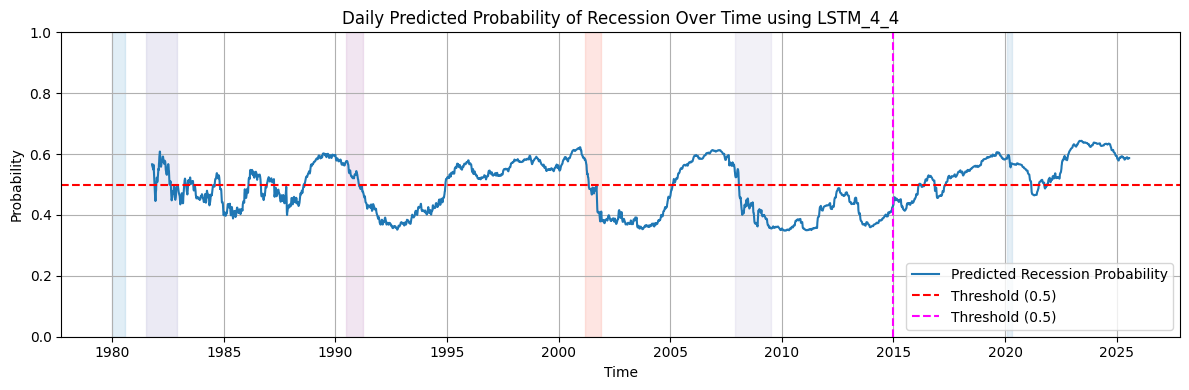
\includegraphics[width=0.31\textwidth]{./Assignment/Final/Steps/Plots/Daily Predicted Probability of Recession Over Time using LSTM_4_4.png} &
        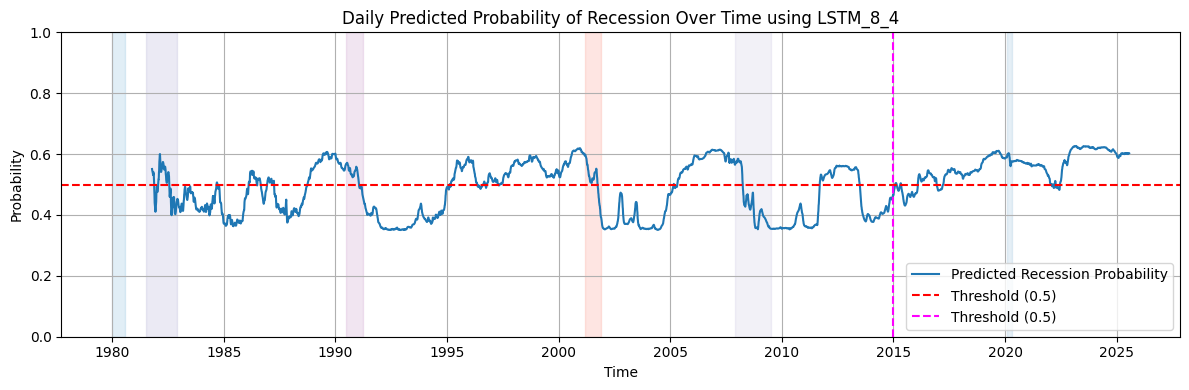
\includegraphics[width=0.31\textwidth]{./Assignment/Final/Steps/Plots/Daily Predicted Probability of Recession Over Time using LSTM_8_4.png} &
        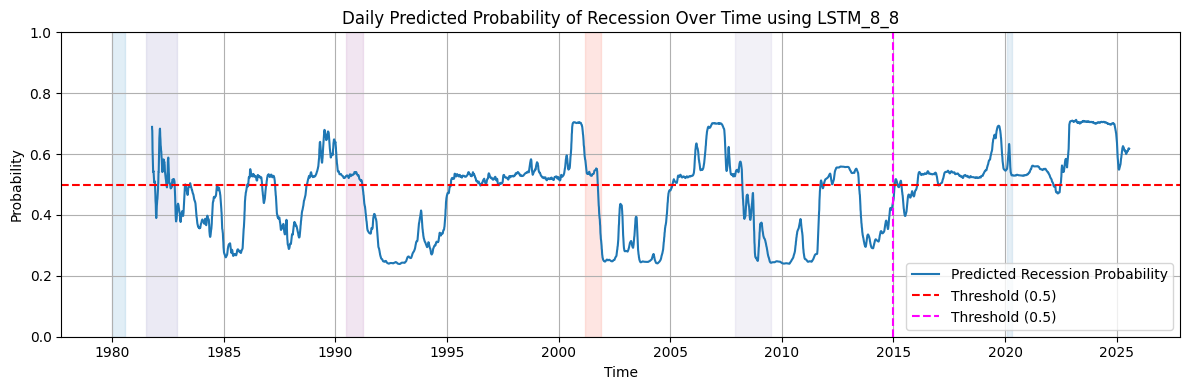
\includegraphics[width=0.31\textwidth]{./Assignment/Final/Steps/Plots/Daily Predicted Probability of Recession Over Time using LSTM_8_8.png} \\ [-9pt]
        %\textbf{Logistic Regression - Daily} & \textbf{Easy Ensemble - Daily} \\
        %\vspace{-9pt}
        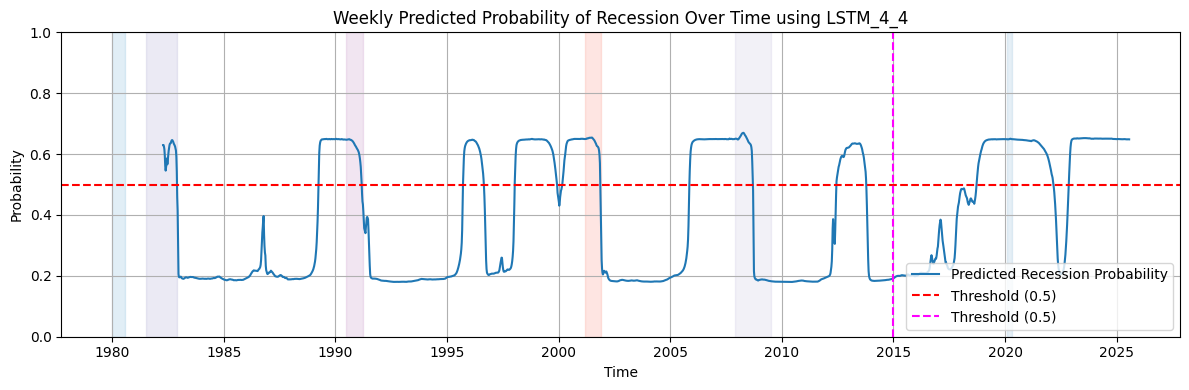
\includegraphics[width=0.31\textwidth]{./Assignment/Final/Steps/Plots/Weekly Predicted Probability of Recession Over Time using LSTM_4_4.png} &
        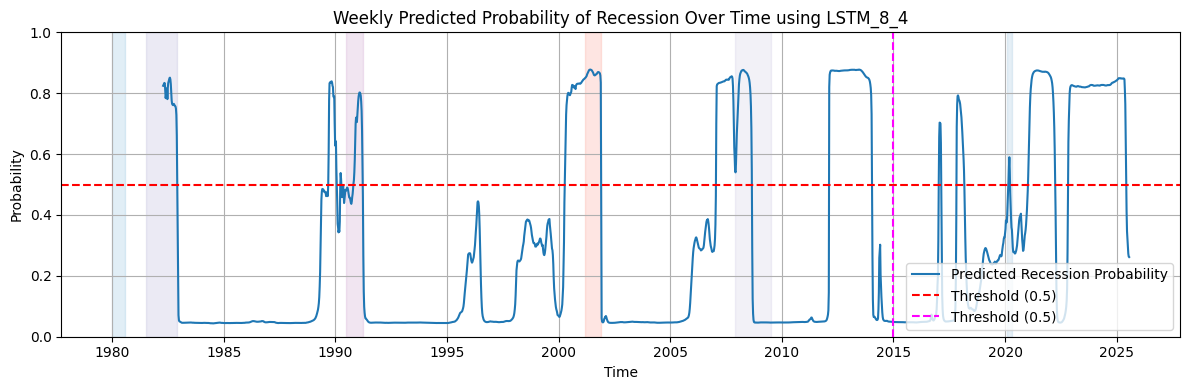
\includegraphics[width=0.31\textwidth]{./Assignment/Final/Steps/Plots/Weekly Predicted Probability of Recession Over Time using LSTM_8_4.png} &
        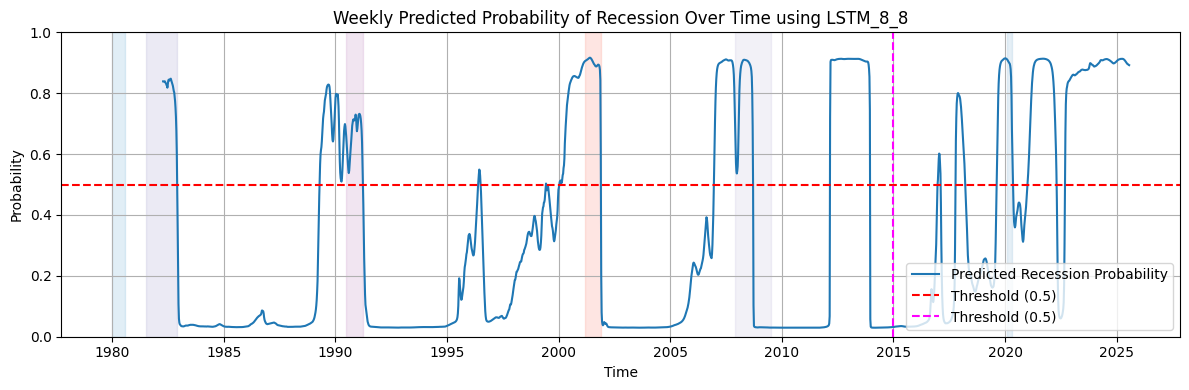
\includegraphics[width=0.31\textwidth]{./Assignment/Final/Steps/Plots/Weekly Predicted Probability of Recession Over Time using LSTM_8_8.png} \\ [-9pt]
        %\textbf{Logistic Regression - Weekly} & \textbf{Easy Ensemble - Weekly} \\
        %\vspace{-9pt}
        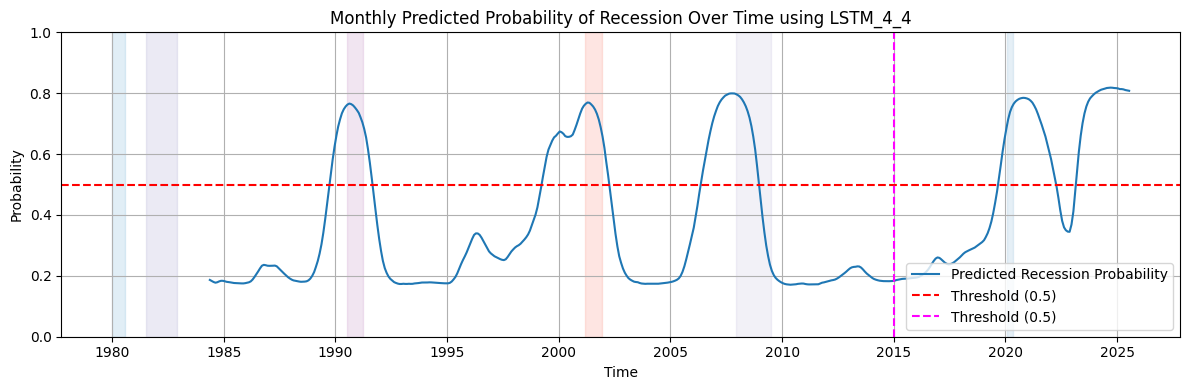
\includegraphics[width=0.31\textwidth]{./Assignment/Final/Steps/Plots/Monthly Predicted Probability of Recession Over Time using LSTM_4_4.png} &
        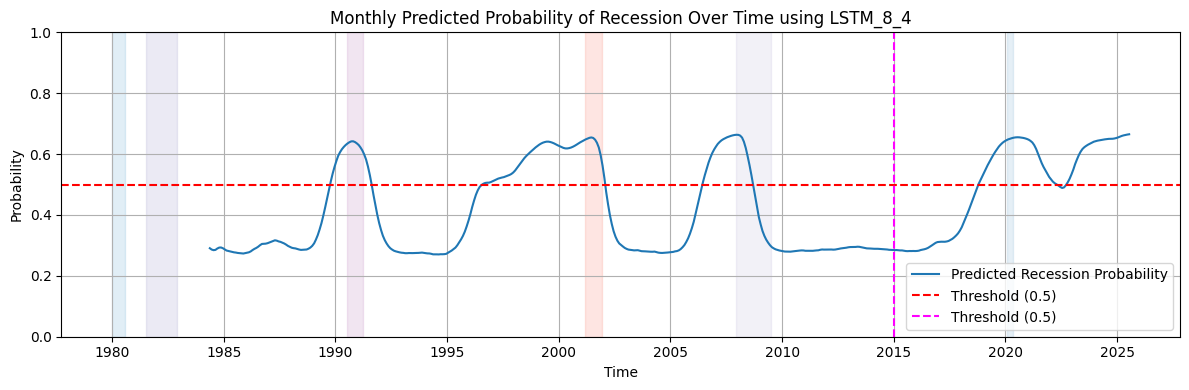
\includegraphics[width=0.31\textwidth]{./Assignment/Final/Steps/Plots/Monthly Predicted Probability of Recession Over Time using LSTM_8_4.png} &
        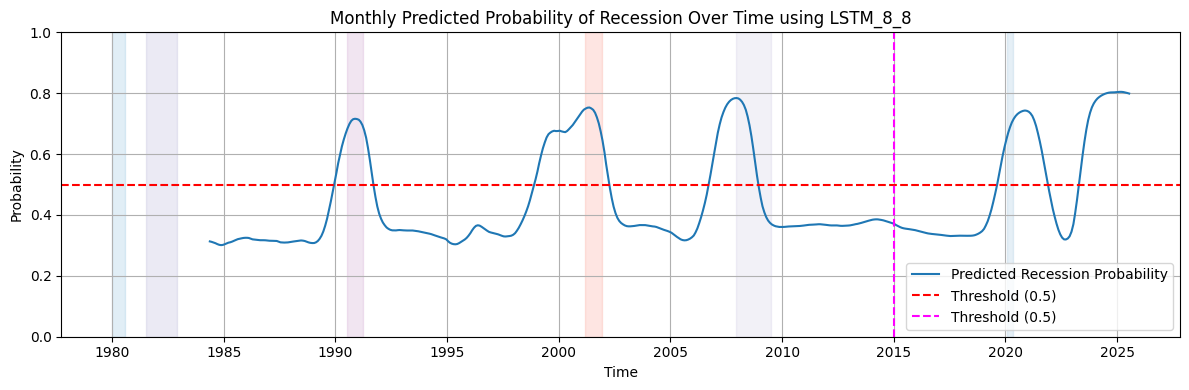
\includegraphics[width=0.31\textwidth]{./Assignment/Final/Steps/Plots/Monthly Predicted Probability of Recession Over Time using LSTM_8_8.png} \\ [-9pt]
        %\textbf{Logistic Regression - Monthly} & \textbf{Easy Ensemble - Monthly} \\
    \end{tabular}
    \caption{Predicted probability of recession %across time frequencies 
    using \LSTMFF (left), \LSTMEF (center) and \LSTMEE (right).}
    \label{fig:table_lstm44_lstm84_lstm88}
\end{figure}



\subsection{Data Interpretation}

\subsubsection{Traditional Model Behavior and Interpretability.}
The strong and consistent performance of Logistic Regression and the Easy Ensemble Classifier across daily, weekly, and monthly datasets highlights their robustness in separating recession signals from background noise. Logistic Regression, in particular, achieved higher \AUCone values, demonstrating that even relatively simple, interpretable models %—when paired with thoughtful feature engineering and class balancing—
can perform competitively in complex economic forecasting tasks. Analysis of the predicted probability trajectories further supports these findings: Logistic Regression tended to produce smoother, more gradual increases in predicted recession risk leading up to historically verified downturns% (e.g., 2001, 2008, 2020)
, making it well-suited for early warning systems where trend clarity and stability are essential. In contrast, the Easy Ensemble Classifier exhibited sharper, more volatile probability spikes. 
This heightened sensitivity may offer advantages in rapidly evolving macroeconomic contexts, though it could also increase the risk of false positives.




\subsubsection{LSTM Model Behavior and Interpretability.}
The performance of LSTM models revealed both potential and pitfalls when applying deep learning to recession forecasting. 
Single-layer LSTMs such as \LSTMF and \LSTME showed reasonable performance. 
With \LSTME achieving the highest AUC among all models at the weekly level. These models were able to capture early signs of recessions with some degree of lead time, validating their ability to model temporal dependencies in sequential economic data. However, they also displayed varying levels of volatility 
suggesting possible sensitivity to noise or overfitting.
Double-layer LSTM models exhibited increased complexity, with \LSTMFF and \LSTMEE striking a favourable balance between signal detection and noise detection across all time frequencies. Although they all perfomred terribly on the weekly dataset (unstable and exaggerated signals, including elevated probabilities during expansionary periods). 


These results reflect a trade-off between model expressiveness and interpretability: while LSTMs are capable of learning complex temporal structures, they require careful regularization and architecture tuning to avoid generating misleading outputs. Notably, the predicted probability plots sometimes diverged from AUC-based evaluations (particularly at monthly frequency) where smoother LSTM outputs may appear more useful for real-time monitoring despite lower AUC values. This underscores a key limitation of AUC as a standalone evaluation metric in time-series classification, as it fails to capture the temporal shape and continuity of prediction trajectories, which are critical in practical forecasting contexts. 
LSTMs demonstrate strong potential in recession forecasting, especially when thoughtfully designed and appropriately trained. Their probabilistic outputs, though less interpretable than those of traditional models, offer valuable flexibility in capturing early warning signals.




\subsection{Unexpected Outcomes}

One of the key unexpected outcomes of this study was the underperformance of the LSTM models relative to the baseline Logistic Regression model. Given the LSTMs’ theoretical advantage in capturing temporal dependencies in sequential data, we expected them to match or exceed the performance of traditional classifiers. However, across most time frequencies, Logistic Regression consistently outperformed LSTM variants in terms of AUC‐ROC. This result challenges the assumption that model complexity necessarily yields superior predictive accuracy in economic time series. Additionally, our findings revealed that AUC‐ROC may not be a fully appropriate metric for evaluating LSTM models in this context. While some LSTM configurations produced informative probability trajectories that aligned well with recession timing, their AUC scores remained relatively low. This discrepancy highlights the limitations of using AUC‐ROC as the sole performance criterion for time-series classification, particularly when sequence shape and trend stability are critical for interpretability and practical use.



